\documentclass{book}
\usepackage{fontspec}
\setmainfont{STIX Two Text}

%PACKAGES
\iffalse
Here are the packages that I use
\fi

\usepackage{blindtext, hyperref, verbatim, minted, graphicx, amssymb, textcomp, enumerate, tcolorbox, newunicodechar, textgreek, wasysym, tipa, eso-pic, lipsum, bbold, dsfont}
\usepackage[margin=1.3in]{geometry}
\usepackage{longtable}
\usepackage{newunicodechar}
\usepackage{amsthm}
\usepackage{tikz}
\usepackage{tikz-cd}






%ENVIRONMENTS

%Here I define some common environments. I use definitions, theorems, examples, and lemmas.


\theoremstyle{definition}
\newtheorem{definition}{Definition}
\newtheorem{theorem}{Theorem}
\newtheorem{example}{Example}
\newtheorem{lemma}{Lemma}


\newunicodechar{ₙ}{${}_{n}$}

\newunicodechar{𝓓}{$\mathcal{D}$}
\newunicodechar{∂}{$\partial$}

%\newunicodechar{π⃗}{$\stackrel{\arr}{\pi}$}

\newunicodechar{×}{$\times$}
\newunicodechar{→}{$\rightarrow$}
\newunicodechar{⟨}{$\langle$}
\newunicodechar{⟩}{$\rangle$}
\newunicodechar{↦}{$\mapsto$}
\newunicodechar{∧}{$\wedge$}
\newunicodechar{∨}{$\vee$}
\newunicodechar{∃}{$\exists$}
\newunicodechar{∀}{$\forall$}
\newunicodechar{¬}{$\neg$}
\newunicodechar{ᵃ}{${}^{\texttt{a}}$}
\newunicodechar{ᵇ}{${}^{\texttt{b}}$}
\newunicodechar{ᶜ}{${}^{\texttt{c}}$}
\newunicodechar{ᵈ}{${}^{\texttt{d}}$}
\newunicodechar{ᵉ}{${}^{\texttt{e}}$}
\newunicodechar{ᶠ}{${}^{\texttt{f}}$}
\newunicodechar{ᵍ}{${}^{\texttt{g}}$}
\newunicodechar{ʰ}{${}^{\texttt{h}}$}
\newunicodechar{ⁱ}{${}^{\texttt{i}}$}
\newunicodechar{ʲ}{${}^{\texttt{j}}$}
\newunicodechar{ᵏ}{${}^{\texttt{k}}$}
\newunicodechar{ˡ}{${}^{\texttt{l}}$}
\newunicodechar{ᵐ}{${}^{\texttt{m}}$}
\newunicodechar{ⁿ}{${}^{\texttt{n}}$}
\newunicodechar{ᵒ}{${}^{\texttt{o}}$}
\newunicodechar{ᵖ}{${}^{\texttt{ω}}$}
\newunicodechar{ʳ}{${}^{\texttt{r}}$}
\newunicodechar{ˢ}{${}^{\texttt{s}}$}
\newunicodechar{ᵗ}{${}^{\texttt{t}}$}
\newunicodechar{ᵘ}{${}^{\texttt{u}}$}
\newunicodechar{ᵛ}{${}^{\texttt{v}}$}
\newunicodechar{ʷ}{${}^{\texttt{w}}$}
\newunicodechar{ˣ}{${}^{\texttt{x}}$}
\newunicodechar{ʸ}{${}^{\texttt{y}}$}
\newunicodechar{ᶻ}{${}^{\texttt{z}}$}
\newunicodechar{⁰}{${}^{\texttt{0}}$}
\newunicodechar{¹}{${}^{\texttt{1}}$}
\newunicodechar{²}{${}^{\texttt{2}}$}
\newunicodechar{³}{${}^{\texttt{3}}$}
\newunicodechar{⁴}{${}^{\texttt{4}}$}
\newunicodechar{⁵}{${}^{\texttt{5}}$}
\newunicodechar{⁶}{${}^{\texttt{6}}$}
\newunicodechar{⁷}{${}^{\texttt{7}}$}
\newunicodechar{⁸}{${}^{\texttt{8}}$}
\newunicodechar{⁹}{${}^{\texttt{9}}$}
\newunicodechar{⁻}{${}^{\texttt{-}}$}
\newunicodechar{ᵒ}{${}^{\texttt{o}}$}
\newunicodechar{ᵖ}{${}^{\texttt{ω}}$}
\newunicodechar{⁻}{${}^{\texttt{-}}$}
\newunicodechar{¹}{${}^{\texttt{1}}$}
\newunicodechar{₀}{${}_{\texttt{0}}$}
\newunicodechar{₁}{${}_{\texttt{1}}$}
\newunicodechar{₂}{${}_{\texttt{2}}$}
\newunicodechar{₃}{${}_{\texttt{3}}$}
\newunicodechar{₄}{${}_{\texttt{4}}$}
\newunicodechar{₅}{${}_{\texttt{5}}$}
\newunicodechar{₆}{${}_{\texttt{6}}$}
\newunicodechar{₇}{${}_{\texttt{7}}$}
\newunicodechar{₈}{${}_{\texttt{8}}$}
\newunicodechar{₉}{${}_{\texttt{9}}$}
\newunicodechar{𝔸}{$\mathbb{A}$}
\newunicodechar{𝔹}{$\mathbb{B}$}
\newunicodechar{ℂ}{$\mathbb{C}$}
\newunicodechar{𝔻}{$\mathbb{D}$}
\newunicodechar{𝔼}{$\mathbb{E}$}
\newunicodechar{𝔽}{$\mathbb{F}$}
\newunicodechar{𝔾}{$\mathbb{G}$}
\newunicodechar{ℍ}{$\mathbb{H}$}
\newunicodechar{𝕀}{$\mathbb{I}$}
\newunicodechar{𝕁}{$\mathbb{J}$}
\newunicodechar{𝕂}{$\mathbb{K}$}
\newunicodechar{𝕃}{$\mathbb{L}$}
\newunicodechar{𝕄}{$\mathbb{M}$}
\newunicodechar{ℕ}{$\mathbb{N}$} 
\newunicodechar{𝕆}{$\mathbb{O}$}
\newunicodechar{ℙ}{$\mathbb{P}$}
\newunicodechar{ℚ}{$\mathbb{Q}$}
\newunicodechar{ℝ}{$\mathbb{R}$}
\newunicodechar{𝕊}{$\mathbb{S}$}
\newunicodechar{𝕋}{$\mathbb{T}$} 
\newunicodechar{𝕌}{$\mathbb{U}$}
\newunicodechar{𝕍}{$\mathbb{V}$}
\newunicodechar{𝕎}{$\mathbb{W}$}
\newunicodechar{𝕏}{$\mathbb{X}$}
\newunicodechar{𝕐}{$\mathbb{Y}$}
\newunicodechar{ℤ}{$\mathbb{Z}$}
\newunicodechar{𝕒}{$\mathbb{a}$}
\newunicodechar{𝕓}{$\mathbb{b}$}
\newunicodechar{𝕔}{$\mathbb{c}$}
\newunicodechar{𝕕}{$\mathbb{d}$}
\newunicodechar{𝕖}{$\mathbb{e}$}
\newunicodechar{𝕗}{$\mathbb{f}$}
\newunicodechar{𝕘}{$\mathbb{g}$}
\newunicodechar{𝕙}{$\mathbb{h}$}
\newunicodechar{𝕚}{$\mathbb{i}$}
\newunicodechar{𝕛}{$\mathbb{j}$}
\newunicodechar{𝕜}{$\mathbb{k}$}%𝔸𝔹ℂ𝔻𝔼𝔽𝔾ℍ𝕀𝕁𝕂𝕃𝕄ℕ𝕆ℙℚℝ𝕊𝕋𝕌𝕍𝕎𝕏𝕐ℤ𝕒𝕓𝕔𝕕𝕖𝕗𝕘𝕙𝕚𝕛𝕜𝕝𝕞𝕟𝕠𝕡𝕢𝕣𝕤𝕥𝕦𝕧𝕨𝕩𝕪𝕫
\newunicodechar{𝕝}{$\mathbb{l}$} 
\newunicodechar{𝕞}{$\mathbb{m}$}
\newunicodechar{𝕟}{$\mathbb{n}$}
\newunicodechar{𝕠}{$\mathbb{o}$}
\newunicodechar{𝕡}{$\mathbb{p}$}
\newunicodechar{𝕢}{$\mathbb{q}$}
\newunicodechar{𝕣}{$\mathbb{r}$}
\newunicodechar{𝕤}{$\mathbb{s}$}
\newunicodechar{𝕥}{$\mathbb{t}$}
\newunicodechar{𝕦}{$\mathbb{u}$}
\newunicodechar{𝕧}{$\mathbb{v}$}
\newunicodechar{𝕨}{$\mathbb{w}$}
\newunicodechar{𝕩}{$\mathbb{x}$}
\newunicodechar{𝕪}{$\mathbb{y}$}
\newunicodechar{𝕫}{$\mathbb{z}$}
\newunicodechar{𝚫}{$\Delta$}
\newunicodechar{ʃ}{$\int$}
\newunicodechar{∪}{$\cup$}
\newunicodechar{∩}{$\cap$}
\newunicodechar{±}{$\pm$}
\newunicodechar{𝔄}{$\mathfrak{A}$}




\newunicodechar{𝔅}{$\mathfrak{B}$}
\newunicodechar{ℭ}{$\mathfrak{C}$}
\newunicodechar{𝔇}{$\mathfrak{D}$}
\newunicodechar{𝔈}{$\mathfrak{E}$}
\newunicodechar{𝔉}{$\mathfrak{F}$}
\newunicodechar{𝔊}{$\mathfrak{G}$}
\newunicodechar{ℌ}{$\mathfrak{H}$}
\newunicodechar{ℑ}{$\mathfrak{I}$}
\newunicodechar{𝔍}{$\mathfrak{J}$}
\newunicodechar{𝔎}{$\mathfrak{K}$}
\newunicodechar{𝔏}{$\mathfrak{L}$}
\newunicodechar{𝔐}{$\mathfrak{M}$}
\newunicodechar{𝔑}{$\mathfrak{N}$}
\newunicodechar{𝔒}{$\mathfrak{O}$}
\newunicodechar{𝔓}{$\mathfrak{P}$}
\newunicodechar{𝔔}{$\mathfrak{Q}$}
\newunicodechar{ℜ}{$\mathfrak{R}$}
\newunicodechar{𝔖}{$\mathfrak{S}$}
\newunicodechar{𝔗}{$\mathfrak{T}$}
\newunicodechar{𝔘}{$\mathfrak{U}$}
\newunicodechar{𝔙}{$\mathfrak{V}$}
\newunicodechar{𝔚}{$\mathfrak{W}$}
\newunicodechar{𝔛}{$\mathfrak{X}$}
\newunicodechar{𝔜}{$\mathfrak{Y}$}
\newunicodechar{ℨ}{$\mathfrak{Z}$}

\newunicodechar{𝔞}{$\mathfrak{a}$}
\newunicodechar{𝔟}{$\mathfrak b$}
\newunicodechar{𝔠}{$\mathfrak{c}$}
\newunicodechar{𝔡}{$\mathfrak{d}$}
\newunicodechar{𝔢}{$\mathfrak{e}$}
\newunicodechar{𝔣}{$\mathfrak{f}$}
\newunicodechar{𝔤}{$\mathfrak{g}$}
\newunicodechar{𝔥}{$\mathfrak{h}$}
\newunicodechar{𝔦}{$\mathfrak{i}$}
\newunicodechar{𝔧}{$\mathfrak{j}$}
\newunicodechar{𝔨}{$\mathfrak{k}$}
\newunicodechar{𝔩}{$\mathfrak{l}$}
\newunicodechar{𝔪}{$\mathfrak{m}$}
\newunicodechar{𝔫}{$\mathfrak{n}$}
\newunicodechar{𝔬}{$\mathfrak{o}$}
\newunicodechar{𝔭}{$\mathfrak{ω}$}
\newunicodechar{𝔮}{$\mathfrak{q}$}
\newunicodechar{𝔯}{$\mathfrak{r}$}
\newunicodechar{𝔰}{$\mathfrak{s}$}
\newunicodechar{𝔱}{$\mathfrak{t}$}
\newunicodechar{𝔲}{$\mathfrak{u}$}
\newunicodechar{𝔳}{$\mathfrak{v}$}
\newunicodechar{𝔴}{$\mathfrak{w}$}
\newunicodechar{𝔵}{$\mathfrak{x}$}
\newunicodechar{𝔶}{$\mathfrak{y}$}
\newunicodechar{𝔷}{$\mathfrak{z}$}

\newunicodechar{𝐀}{${\bf{A}}$}
\newunicodechar{𝐁}{${\bf{B}}$}
\newunicodechar{𝐂}{${\bf{C}}$}
\newunicodechar{𝐃}{${\bf{D}}$}
\newunicodechar{𝐄}{${\bf{E}}$}
\newunicodechar{𝐅}{${\bf{F}}$}
\newunicodechar{𝐆}{${\bf{G}}$}
\newunicodechar{𝐇}{${\bf{H}}$}
\newunicodechar{𝐈}{${\bf{I}}$}
\newunicodechar{𝐉}{${\bf{J}}$}
\newunicodechar{𝐊}{${\bf{K}}$}
\newunicodechar{𝐋}{${\bf{L}}$}
\newunicodechar{𝐌}{${\bf{M}}$}
\newunicodechar{𝐍}{${\bf{N}}$}
\newunicodechar{𝐎}{${\bf{O}}$}
\newunicodechar{𝐏}{${\bf{P}}$}
\newunicodechar{𝐐}{${\bf{Q}}$}
\newunicodechar{𝐑}{${\bf{R}}$}
\newunicodechar{𝐒}{${\bf{S}}$}
\newunicodechar{𝐓}{${\bf{T}}$}
\newunicodechar{𝐔}{${\bf{U}}$}
\newunicodechar{𝐕}{${\bf{V}}$}
\newunicodechar{𝐖}{${\bf{W}}$}
\newunicodechar{𝐗}{${\bf{X}}$}
\newunicodechar{𝐘}{${\bf{Y}}$}
\newunicodechar{𝐙}{${\bf{Z}}$}

\newunicodechar{𝐚}{${\bf{a}}$}
\newunicodechar{𝐛}{${\bf{b}}$}
\newunicodechar{𝐜}{${\bf{c}}$}
\newunicodechar{𝐝}{${\bf{d}}$}
\newunicodechar{𝐞}{${\bf{e}}$}
\newunicodechar{𝐟}{${\bf{f}}$}
\newunicodechar{𝐠}{${\bf{g}}$}
\newunicodechar{𝐡}{${\bf{h}}$}
\newunicodechar{𝐢}{${\bf{i}}$}
\newunicodechar{𝐣}{${\bf{j}}$}
\newunicodechar{𝐤}{${\bf{k}}$}
\newunicodechar{𝐥}{${\bf{l}}$}
\newunicodechar{𝐦}{${\bf{m}}$}
\newunicodechar{𝐧}{${\bf{n}}$}
\newunicodechar{𝐨}{${\bf{o}}$}
\newunicodechar{𝐩}{${\bf{ω}}$}
\newunicodechar{𝐪}{${\bf{q}}$}
\newunicodechar{𝐫}{${\bf{r}}$}
\newunicodechar{𝐬}{${\bf{s}}$}
\newunicodechar{𝐭}{${\bf{t}}$}
\newunicodechar{𝐮}{${\bf{u}}$}
\newunicodechar{𝐯}{${\bf{v}}$}
\newunicodechar{𝐰}{${\bf{w}}$}
\newunicodechar{𝐱}{${\bf{x}}$}
\newunicodechar{𝐲}{${\bf{y}}$}
\newunicodechar{𝐳}{${\bf{z}}$}

\newunicodechar{⊣}{\ensuremath{\dashv}}
\newunicodechar{ॱ}{${}^{\cdot}$}
\newunicodechar{𛲔}{${}_{\cdot}$}
\newunicodechar{⋯}{$\cdots$}
\newunicodechar{⇄}{$\rightleftarrows$}
\newunicodechar{⇆}{$\leftrightarrows$}

\newunicodechar{ꜝ}{$\raisebox{1ex}{\scalebox{0.5}{\texttt{!}}}$}
\newunicodechar{ꜞ}{$\raisebox{1ex}{\scalebox{0.5}{\texttt{¡}}}$}



%This is notation we will use for categories


\newunicodechar{𝟙}{$\mathbb{1}$}
\newunicodechar{∘}{$\circ$}

%This is notation we will use for twocategories


\newunicodechar{𝟏}{${\bold{1}}$}
\newunicodechar{⭢}{$\longrightarrow$}
\newunicodechar{•}{${\bullet}$}
\newunicodechar{∙}{${\bullet}$}

%This is notation we will use for ∞-ℂ𝕒𝕥

\newunicodechar{よ}{$
\includegraphics[width=0.27cm,height=0.27cm]{yon.png}$}
\newunicodechar{⊥}{$\bot$}
\newunicodechar{∼}{$\sim$}
\newunicodechar{≃}{$\simeq$}
\newunicodechar{≅}{$\cong$}
\newunicodechar{∞}{$\infty$}

\newunicodechar{α}{$\alpha$}
\newunicodechar{β}{$\beta$}
\newunicodechar{γ}{$\gamma$}
\newunicodechar{δ}{$\delta$}
\newunicodechar{ε}{$\epsilon$}
\newunicodechar{η}{$\eta$}
\newunicodechar{ζ}{$\zeta$}
\newunicodechar{θ}{$\theta$}
\newunicodechar{ι}{$\iota$}
\newunicodechar{μ}{$\mu$}
\newunicodechar{κ}{$\kappa$}
\newunicodechar{λ}{$\lambda$}
\newunicodechar{ρ}{$\rho$}
\newunicodechar{π}{$\pi$}
\newunicodechar{σ}{$\sigma$}
\newunicodechar{τ}{$\tau$}
\newunicodechar{υ}{$\upsilon$}
\newunicodechar{φ}{$\phi$}
\newunicodechar{ψ}{$\psi$}
\newunicodechar{ξ}{$\xi$}
\newunicodechar{χ}{$\chi$}
\newunicodechar{ω}{$\omega$}

\newunicodechar{⊗}{$\otimes$}

\makeatletter
\newcommand*{\shifttext}[2]{\settowidth{\@tempdima}{#2}\makebox[\@tempdima]{\hspace*{#1}#2}}
\makeatother
\definecolor{Red}{cmyk}{0.1, 0.70, 0.65, 0.00, 1.00}
\definecolor{Blue}{cmyk}{0.9, 0.2, 0.2, 0.00, 1.00}
\definecolor{Yellow}{cmyk}{0.0, 0.00, 0.7, 0.00, 0.5}
\definecolor{Green}{cmyk}{0.6, 0.0, 0.6, 0.00, 1.00}
\definecolor{Purple}{cmyk}{0.8, 0.3, 0.3, 0.00, 1.00}
\definecolor{Orange}{cmyk}{0.0, 0.3, 0.7, 0.00, 1.00}
\definecolor{Grey}{cmyk}{0.13, 0.13, 0.13, 0.00, 1.00}
\newcounter{definitioncounter}
\setcounter{definitioncounter}{1}
\newcounter{theoremcounter}
\setcounter{theoremcounter}{1}
\newcounter{printcounter}
\setcounter{printcounter}{1}
\newcounter{examplecounter}
\setcounter{examplecounter}{1}
\newcounter{ccounter}
\setcounter{ccounter}{1}
\newcounter{pcounter}
\setcounter{pcounter}{1}
\newcounter{lcounter}
\setcounter{lcounter}{1}
\newcounter{sectioncount}
\newcounter{subsectioncount}
\setcounter{sectioncount}{1}
\renewcommand{\section}[1]{\newpage\ \\ \ \\ \begin{center} \scalebox{1.5}{\texttt{\thesectioncount . #1}} \stepcounter{sectioncount} \setcounter{subsectioncount}{1} \end{center} \begin{center} \ \\ \ \\ \thispagestyle{empty} \end{center}}
\renewcommand{\subsection}[1]{\texttt{\thesubsectioncount . #1} \stepcounter{subsectioncount}}
\renewcommand{\backslash}{\reflectbox{\texttt{/}}}

\newcounter{chaptercount}
\renewcommand{\chapter}[1]{
\newpage
{
\Huge 
\begin{center}
\ \\
\ \\
\thispagestyle{empty}
\texttt{#1}
\end{center}}
\ \\
\ \\
}

\newcounter{partcount}
\stepcounter{partcount}
\renewcommand{\part}[1]{
\newpage
{
\Huge 
\begin{center}
\ \\
\ \\
\ \\
\ \\
\ \\
\ \\
\thispagestyle{empty}
\texttt{PART {\thepartcount}: #1}
\stepcounter{partcount}
\end{center}}
\ \\
\ \\
}


\begin{document}

\thispagestyle{empty} 

\AddToShipoutPicture*
    {\put(540,720){

    \href{http://www.linearlibrary.net}{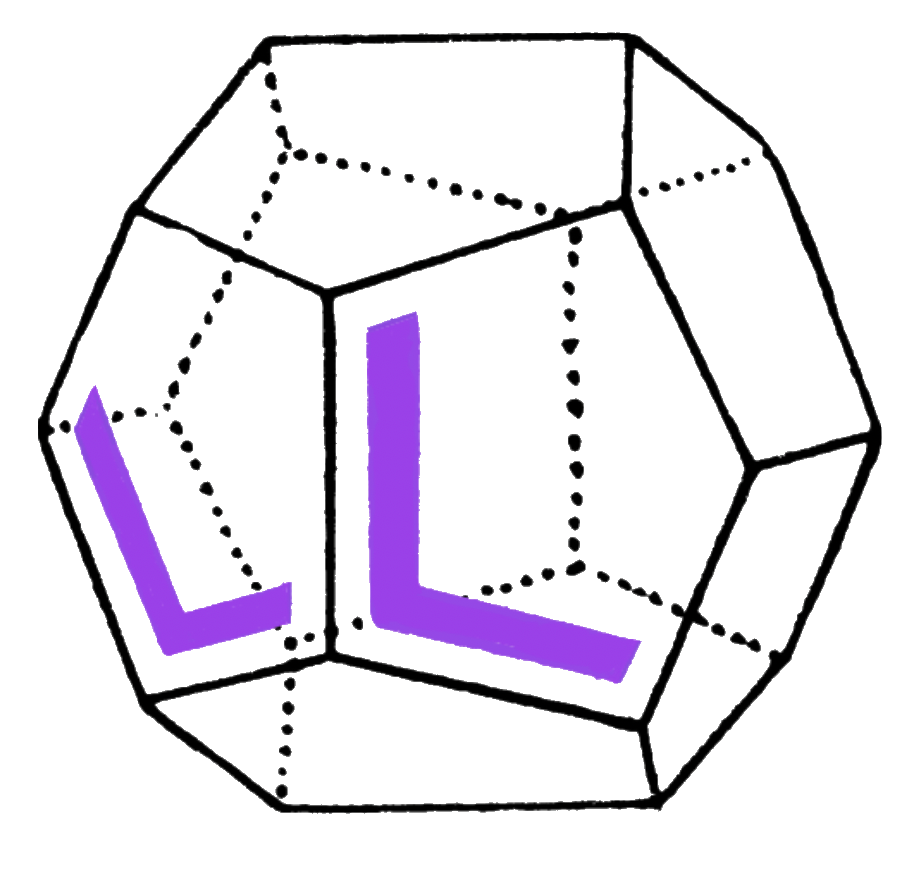
\includegraphics[width=2cm,height=2cm]{ll.png}}

    }}

\AddToShipoutPicture*
  {\put(470,767){
    \href{https://github.com/linlib/CategoriesandHilbertSpaces/StringDiagramGenerator.py}{\texttt{.py file}}
  }}

\AddToShipoutPicture*
  {\put(470,752){
    \href{https://github.com/linlib/ThreeWhiteheadTheoremsandThreePuppeSequences/ThreeWhiteheadTheoremsandThreePuppeSequences.tex}{\texttt{.tex file}}\\

  }}


\AddToShipoutPicture*
  {\put(470,737){

    \href{http://linearlibrary.net/ThreeWhiteheadTheoremsandThreePuppeSequences/ThreeWhiteheadTheoremsandThreePuppeSequences.pdf}{\texttt{.pdf file}}\\

  }}

  \AddToShipoutPicture*
  {\put(470,722){
    \href{https://github.com/linlib/ThreeWhiteheadTheoremsandThreePuppeSequences/ThreeWhiteheadTheoremsandThreePuppeSequences.lean}{\texttt{.lean file}}

  }}

\ \\

%LEAN: 
\begin{center}
\begin{tcolorbox}[width=5.8in,colback={white},coltitle=white]
\begin{center}
\ \\
\scalebox{3}{\texttt{∞-Spaces}}\\
\ \\
\end{center}
\end{tcolorbox}
\end{center}
\ \\
{\footnotesize
\begin{center}
\scalebox{1.1}{
\begin{tabular}{|| l | l || l | l | l  || l | l || l | l | l  || } 
\hline
$\texttt{Mon}$ & \texttt{D(}∞\texttt{-Cat)} & Σ⃗ & Ω⃗ & P⃗ & $\texttt{InfPreShf}$ & \texttt{D(}∞\texttt{-Cat/C)} & σ⃗ & ω⃗ & p⃗ \\
\hline
$\texttt{ComMon}$ & \texttt{D(}∞\texttt{-Grpd)} & Σ⃡ & Ω⃡ & P⃡  & $\texttt{IntAct}$ & \texttt{D(}∞\texttt{-Grpd/G)} & σ⃡ & ω⃡ & p⃡\\
 \hline
$\texttt{IntGrp}$ & \texttt{D(}∞\texttt{-Grpd₀)} & Σ & Ω & P  & $\texttt{IntAct₀}$ & \texttt{D(}∞\texttt{-Grpd₀/G₀)} & σ & ω & p \\
 \hline
\end{tabular}}
\end{center}}
\ \\
%LEAN: 
\begin{center}
\begin{tcolorbox}[width=6in,colback={white}]
\begin{center}
\ \\
\end{center}
\end{tcolorbox}
\end{center}

%LEAN: 
\begin{center}
\begin{tcolorbox}[width=4.13in,colback={white},coltitle=white]
\scalebox{1.5}{E. Dean Young}
\end{tcolorbox}
\end{center}


\begin{center}
\texttt{Plans to prove three variations of the}\\
\texttt{Whitehead theorem of homotopy groups in}\\
\texttt{Lean 4, with extensive use of Mathlib 4}
\end{center}


\thispagestyle{empty}


\newpage


\begin{center}

\pagecolor{white}
\color{black}




\end{center}

\thispagestyle{empty}




\newpage
\pagecolor{white}
\color{black}
\ \\
\ \\
\thispagestyle{empty}
\begin{center}
Copyright\ \textcopyright \ October 19th 2023 Elliot Dean Young and Jiazhen Xia.\ All rights reserved.\\
\end{center}
\large %%%%%%%% HERE IS THE large LARGE size textsize set text size
\newpage 
\ \\
\ \\
\ \\
\ \\
\ \\
\ \\
\ \\
\ \\
\ \\
\ \\
\ \\
\thispagestyle{empty}
 
\newpage

\ \\
\ \\
\ \\
\ \\
\ \\
\ \\
\ \\
\ \\
\ \\
\ \\
\ \\

We wish to acknowledge the collaborative efforts of E. Dean Young and Jiazhen Xia. Dean Young initially formulated the introduction with twelve goals, posting them on the Lean Zulip in August of 2023. Together the authors are pursuing these plans as a long term project.\\



\newpage



\newpage



\section{Introduction}

In this document I would like to explore derivations and connections.\\

\begin{enumerate}
\item Derivations
\item Connections
\end{enumerate}

In this section, which makes use of the previous section concerning Haar integral, I intend to cover the ordinary versions of Poincare duality, Pontrjagin duality, and Fourier duality, as well as versions of these theorems using language enabled by the previous repositories. This won't culminate until far into the future, so for now I have jotted down some sketches.\\

I begin by considering the concept of a finite extension, as well as the separable closure and the maximal unramified extension. This will be used in developing the main example in what ensues. Here is a tentative list of sections:\\




\section{Contents}

\iffalse
{
\footnotesize
\begin{longtable}{|| l || l ||} 
\hline
\multicolumn{1}{||c||}{$\texttt{Section}$} & \multicolumn{1}{|c||}{$\texttt{Description}$} \\
\hline
\hline
Unfinished & \\
\hline
Contents & \\
\hline
Unicode & \\
\hline
Introduction & \\
\hline \hline
\multicolumn{2}{||c||}{\texttt{PART I: } ABELIAN GROUPS AND ∞-SPACES} \\
\hline \hline
 \multicolumn{2}{||c||}{\texttt{Chapter 1: }Abelian Groups} \\
\hline \hline
 &  \\
\hline \hline
 \multicolumn{2}{||c||}{\texttt{Chapter 2: }Tensor Product of Abelian Groups} \\
\hline \hline
 &  \\
 \hline \hline
 \multicolumn{2}{||c||}{\texttt{Chapter 3: }Rings and Modules} \\
\hline \hline
 &  \\
 \hline \hline
 \multicolumn{2}{||c||}{\texttt{Chapter 4: }∞-Spaces} \\
\hline \hline
 &  \\
\hline \hline
 \multicolumn{2}{||c||}{\texttt{Chapter 5: }Tensor Product of ∞-Spaces} \\
\hline \hline
 &  \\
 \hline \hline
  \multicolumn{2}{||c||}{\texttt{Chapter 6: }∞-Rings and ∞-Modules} \\
\hline \hline
 &  \\
 \hline \hline
 \multicolumn{2}{||c||}{\texttt{Chapter 7: }Free ∞-Rings and ∞-Modules} \\
\hline \hline
 &  \\
\hline \hline
\multicolumn{2}{||c||}{\texttt{PART II: } Based connected ∞-groupoids} \\
\hline \hline
\hline \hline
\end{longtable}
}
\fi


\iffalse
https://redprl.org/
agda
rzk (new!)

Filippo A. E. Nuccio: Hi Dean, thanks for reaching out! I have had a brief look at your pdf and your lean code. Can you give some more details about your project, what you are exactly aiming at (integrating mathlib? writing a book on your own? writing a thesis to showcase your Lean expertise to apply for grad fellowship)? In particular, how can I provide feedback exactly?

Dean Young: Sorry for my late reply Filippo.

My collaborator (Jiazhen Xia) and I have a main goal of making a Mathlib PR. It would be helpful to get tips, points of importance, and suggestions for changes that would make it more likely to be accepted. We've set aside about a year to work through it, and we're taking the time to make as many changes as we need to ensure things like usability.

Separately, if you feel comfortable recommending me on this basis to PhD programs as well, it would improve the strength of my applications by a lot.

Dean Young: The most important kind of feed back is, what are some considerations in making the Whitehead theorem and Puppe sequence things that people would use? We are especially interested in this from the perspective of algebraic geometry.

Filippo A. E. Nuccio: Dear Dean, it is my turn to apologise for a late reply. I have seen your project and it is huge: I think that if you want to reasonably complete in a finite amount of time and to start doing PR's you should really identify a first much smaller goal.

Filippo A. E. Nuccio: I am not an expert in algebraic topology "in the modern sense", I would love to see the Whitehead theorem spelt down in purely topological terms, and this would certainly be a result in its own without the "need" for any application.

Filippo A. E. Nuccio: On the other hand, I see things that are already in mathlib, like pullback and pushouts: are you aware that you won't need to develop them?

Filippo A. E. Nuccio: The take-home message is really: start with a very small PR. Huge ones are hard to check, and if you got something wrong you'd rather discover it sooner than later.

Filippo A. E. Nuccio: If you want to continue the discussion, I would suggest that

You identify this small contribution, even if on the very long run you are aiming at Whitehead/Puppe
You discuss this small contribution in the public chat
You strive for it and try to make this first small PR. If it works, you'll make a second one. I was involved in LTE and one of the reasons it will be difficult to make a global PR is that it is too big and many things have diverged from themaster version of mathlib.
Filippo A. E. Nuccio: Concening your PhD, can I ask more details? Where are you based, where would you like to look for programs, have you a math/CS background, what is your primary scientific interest, how long is your NYU program?
\fi

\iffalse
https://mathoverflow.net/questions/464176/bⁿ-and-coherence
\fi


after this we develop chain complexes of these.\\


The table of contents below reflects the tentative long-term goals of the authors, with the main goal the pursuit of the Whitehead theorem for a point-set model involving Mathlib's predefined homotopy groups.\\

\begin{enumerate}
\item cup and cap product
\end{enumerate}

Ideas for future applications:

\begin{enumerate}
\item \url{https://arxiv.org/pdf/2206.13563.pdf}
\end{enumerate}

\begin{enumerate}
\item One of the basic things I wanted out of this was homotopy colimit preserving maps (Eⁱⁿᶠ-Alg A)ᵒᵖ ⭢ ∞-Grpd
\end{enumerate}


\part{PART I: ABELIAN GROUPS AND ∞-SPACES}

{
\footnotesize
\begin{center}
\begin{tabular}{||l || l || l || l ||} 
 \hline
  \multicolumn{4}{||c||}{\texttt{Eight Structures}} \\
 \hline
 \multicolumn{2}{||c||}{\texttt{Strict}}  &  \multicolumn{2}{||c||}{\texttt{Lax}} \\
 \hline
 \texttt{Unitial} &  \texttt{Actional}  &  \texttt{Unitial} &  \texttt{Actional}\\
 \hline \hline
 \texttt{InternalMonoid}  & \texttt{InternalMonoidAction} & \texttt{OperadicMonoid} & \texttt{OperadicMonoidAction} \\ 
 \hline
 \texttt{InternalCommutative Monoid} & \texttt{InternalCommutativeMonoidAction} & \texttt{OperadicMonoid} & \texttt{OperadicMonoidAction} \\ 
 \hline
 \hline
\end{tabular}
\end{center}
}


\chapter{Abelian Groups}

Abelian groups are internal groups in internal groups.



\chapter{Tensor Product of Abelian Groups}




\chapter{Rings and Modules}

make sure to include Alg




\chapter{∞-Spaces}

\iffalse
OperadicCategory² ∞-Cat, OperadicGroupoid² ∞-Grpd, and OperadicGroup² ∞-Grpd
\fi


\begin{enumerate}
\item OperadicCategory², OperadicGroupoid², OperadicGroup²
\end{enumerate}


Could ∞-spaces be operadic groups in operadic groups?



\iffalse
B.obj (M × N) ⭢ (B.obj M) × (B.obj N)

gives
"the little squares operad"

\fi


\chapter{Tensor Product of ∞-Spaces}




\chapter{∞-Rings and ∞-Modules}

\iffalse
Besides that my ∞-spaces are different, I would like to make my Ainfinity and Einfinity objects as similar as possible.
\fi


make sure to include ∞-Alg...





\part{PART II: FREE ∞-RINGS AND FREE ∞-MODULES}

{
\footnotesize
\begin{center}
\begin{tabular}{||l ||} 
 \hline
 \hline
Set ⇄ AbelianGroup \\
 \hline
∞-Grpd ⇄ ∞-Space \\
 \hline 
 \hline
Ring ⇄ ∞-Ring \\
 \hline
Mod R ⇄ ∞-Mod R \\
 \hline
 \hline
\end{tabular}
\end{center}
}


\chapter{∞-Grpd ⇄ ∞-Space}



\begin{enumerate}
\item πₙ of an ∞-space arising from an ∞-groupoid vs. Hₙ of 
\item 
\end{enumerate}


\chapter{Ring ⇄ ∞-Ring}

\iffalse
Λ*... use a subscript with round braces for the strict and lax variations
Ω as well
λ for actional
ω for actional
\fi


\chapter{Mod R ⇄ ∞-Mod R}

\iffalse
Λ*... use a subscript with round braces for the strict and lax variations
Ω as well
λ for actional
ω for actional
\fi



\part{PART III: DERIVATIONS AND CONNECTIONS}

{
\footnotesize
\begin{center}
\begin{tabular}{|| l || l ||} 
\hline
(Alg R)/B ⇄ Mod B  & (∞-Alg R)/B ⇄ ∞-Mod B \\
 \hline 
??? ⇄ ???  & ??? ⇄ ??? \\
 \hline
\end{tabular}
\end{center}
}

\iffalse
https://en.wikipedia.org/wiki/Connection_(vector_bundle)
\fi


\chapter{Lie Algebras}




\chapter{Lie Algebra Representations}





\chapter{Derivations}

\begin{enumerate}
\item I would like to first construct the lie-algebra of derivations using the spectrum \texttt{Ωⁱⁿᶠ.obj X}. It seems related to coalgebra endomorphisms from \texttt{Ωⁱⁿᶠ.obj X} to itself.\\
\item Lie algebras and Derₖ(A,A)
\end{enumerate}


\chapter{Connections}

\begin{enumerate}
\item I would like to first construct the lie-algebra representation of flat connections using the spectrum \texttt{ωⁱⁿᶠ.obj X).obj V}.
\item \iffalse https://en.wikipedia.org/wiki/Connection_(vector_bundle)\fi
\item Lie algebra representations and ...
\item \\
\item We can define differentiable and connective functionals in this context as well.
\item \iffalse https://en.wikipedia.org/wiki/Connection_(vector_bundle)\fi
\item Somehow connections are the dual of the free abelian group action
\end{enumerate}


\iffalse
https://en.wikipedia.org/wiki/Connection_form
\fi





    \iffalse
    https://amathew.wordpress.com/2011/05/14/the-cotangent-complex-i-group-objects-in-categories-of-algebras/
    \fi



    \iffalse
    I loaded them up onto degree negative one.
    \fi



    Some goals:
    \begin{enumerate}
    \item 
    \end{enumerate}

    \begin{enumerate}
    \item smooth (etale locally ???)
    \item analytic (etale locally ???)
    \item [ℂP¹,ℂP¹] ≅ ℂ(x)
    \item Our ℝ is ∂.obj ℤ regarded as an object in [γ⃗,∞\_(∞-Grpd)]
    \item B.obj det : B.obj U(n) ⭢ B.obj U(1)
    \item Which E${}_{\infty}$ Space have a Chern class?
    \end{enumerate}

    Cohomology with coefficients in $\texttt{[-,Bℂˣ]}$ plays a .\\

    \iffalse
    https://www.universiteitleiden.nl/binaries/content/assets/science/mi/scripties/bachbecker.pdf
    \fi

\begin{enumerate}
\item \iffalse https://en.wikipedia.org/wiki/Connection_(vector_bundle) \fi
\item d2 is wedge with 
\end{enumerate}



\chapter{L${}^{\infty}$ Algebras}




\chapter{L${}^{\infty}$ Algebra Representations}





\chapter{∞-Derivations}




\chapter{∞-Connections}





\newpage

\chapter{Bibliography}

\begin{enumerate}
\item Samuel Eilenberg and Saunders Mac Lane, "On the Groups H(π, n). I", Annals of Mathematics, Second Series, Vol. 58, No. 1 (Jul., 1953), pp. 55-106.
\item Samuel Eilenberg and Saunders Mac Lane, "On the Groups H(π, n). II", Annals of Mathematics, Second Series, Vol. 60, No. 1 (Jul., 1954), pp. 49-139.
\item Saunders Mac Lane, "On the Homology Theory of Eilenberg-Mac Lane", Proceedings of the National Academy of Sciences of the United States of America, Vol. 35, No. 11 (Nov. 15, 1949), pp. 657-663.
\item Eilenberg, S., & MacLane, S. (1945). Relations Between Homology and Homotopy Groups of Spaces. Proceedings of the National Academy of Sciences of the United States of America, 31(2), 83–87. 
\end{enumerate}



\newpage 
\ \\
\ \\
\ \\
\ \\
\ \\
\ \\
%LEAN: 
\begin{center}
\begin{tcolorbox}[width=5in,colback={white},title={\begin{center}\texttt{About the Author} \addtocounter{lcounter}{1}  \end{center}},colbacktitle=Yellow,coltitle=black]
Dean Young is a master's student at New York University, where he studies mathematics. \\
\begin{center}
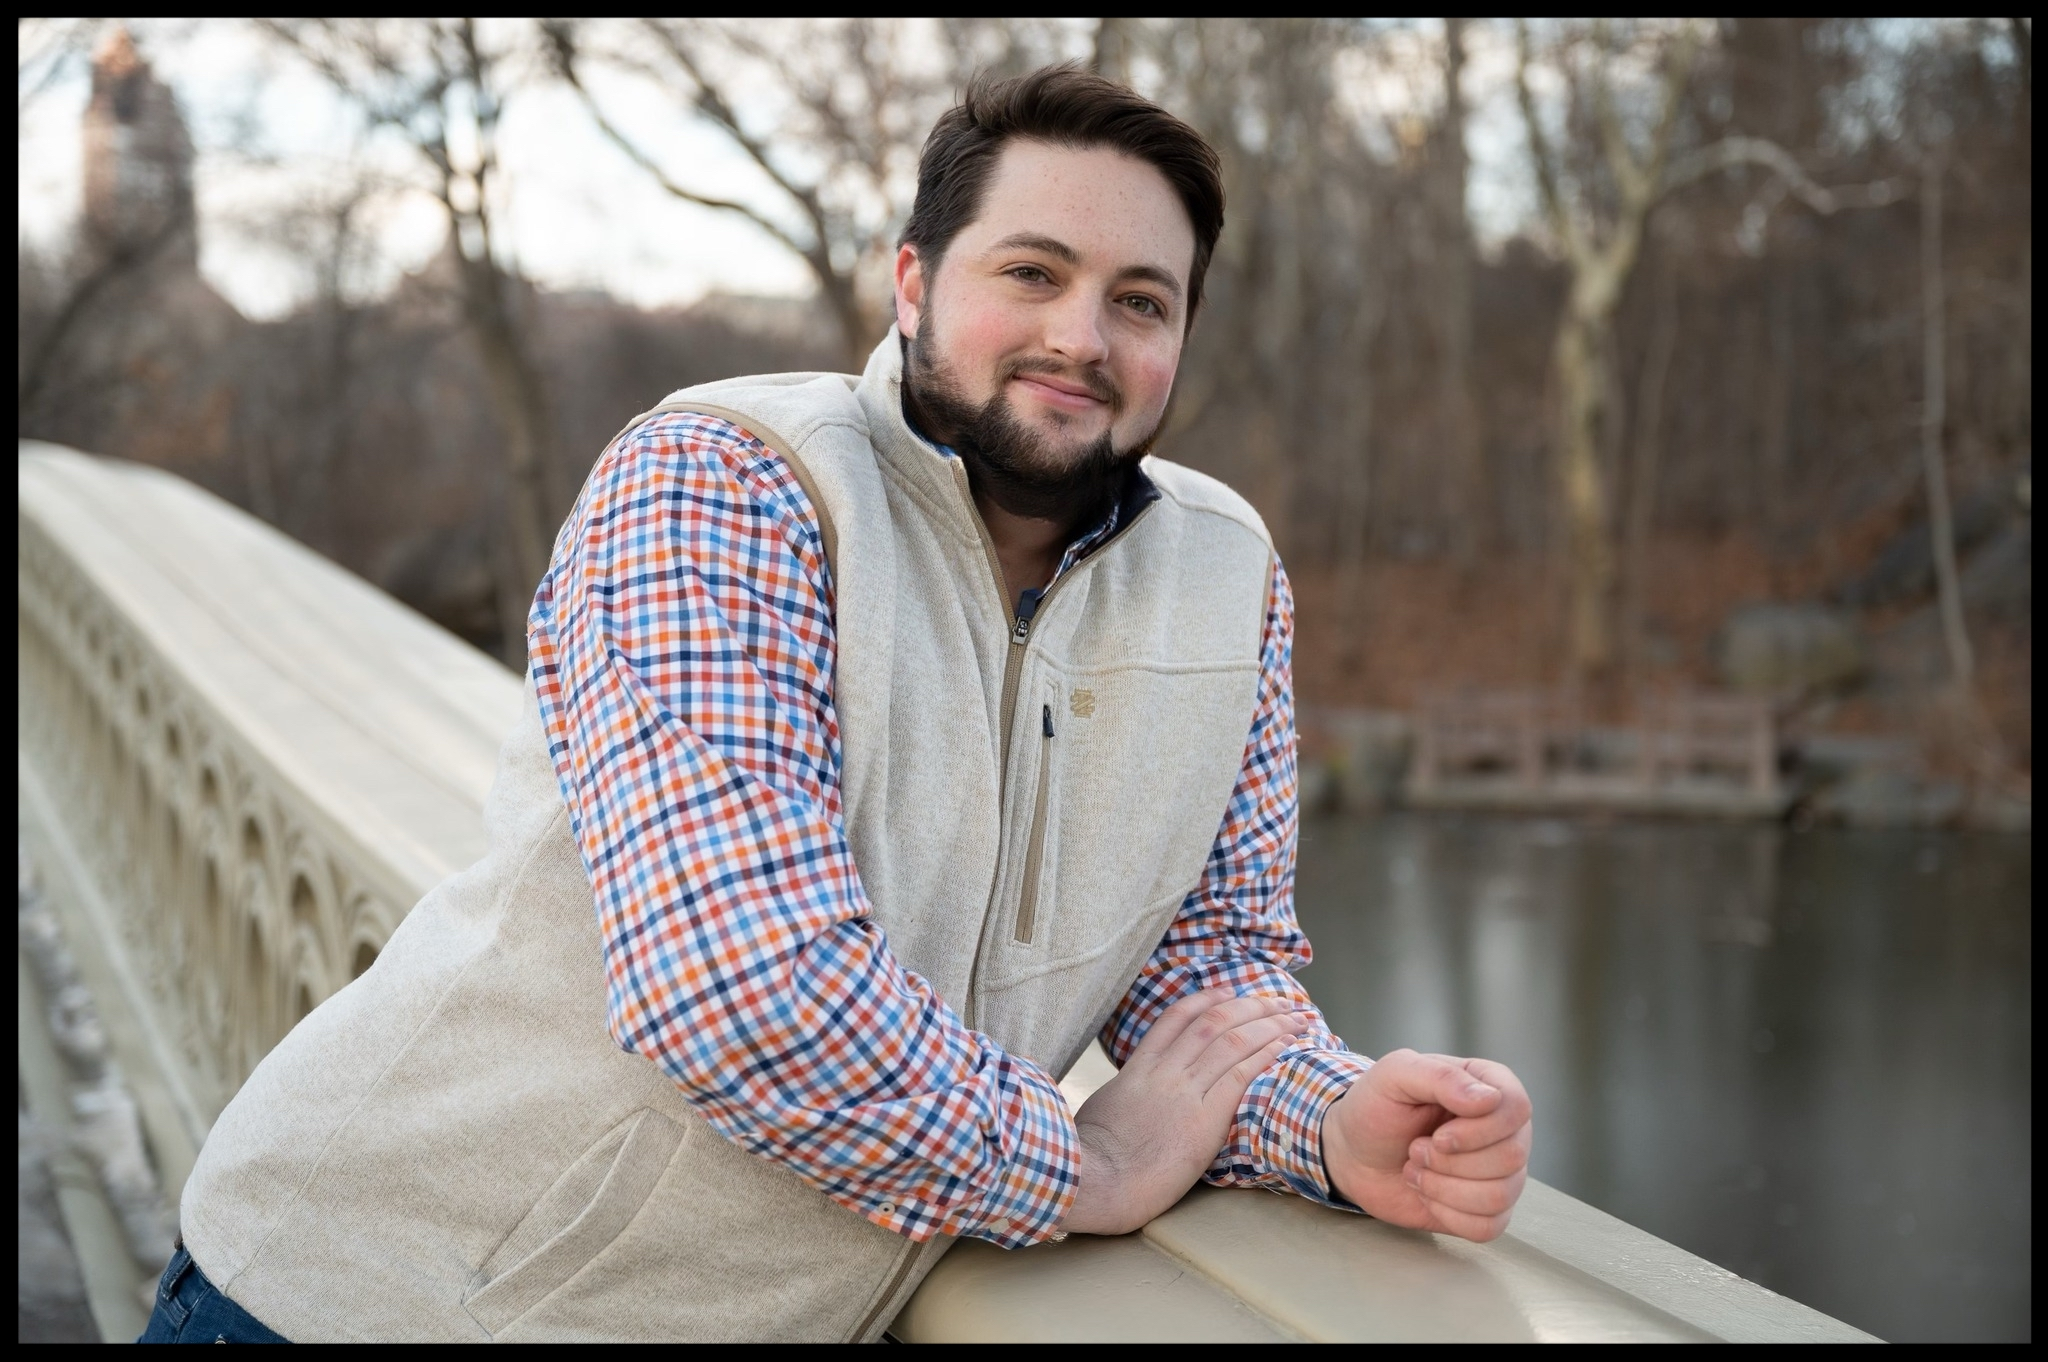
\includegraphics[width=7.5cm,height=5cm]{about.jpg}
\end{center}
\end{tcolorbox}
\end{center}

\begin{center}
\begin{tcolorbox}[width=5in,colback={white},title={\begin{center}\texttt{About the Author} \addtocounter{lcounter}{1}  \end{center}},colbacktitle=Yellow,coltitle=black]
Jiazhen Xia is a master's student at Zhejiang University, where he studies computer science. \\
\begin{center}
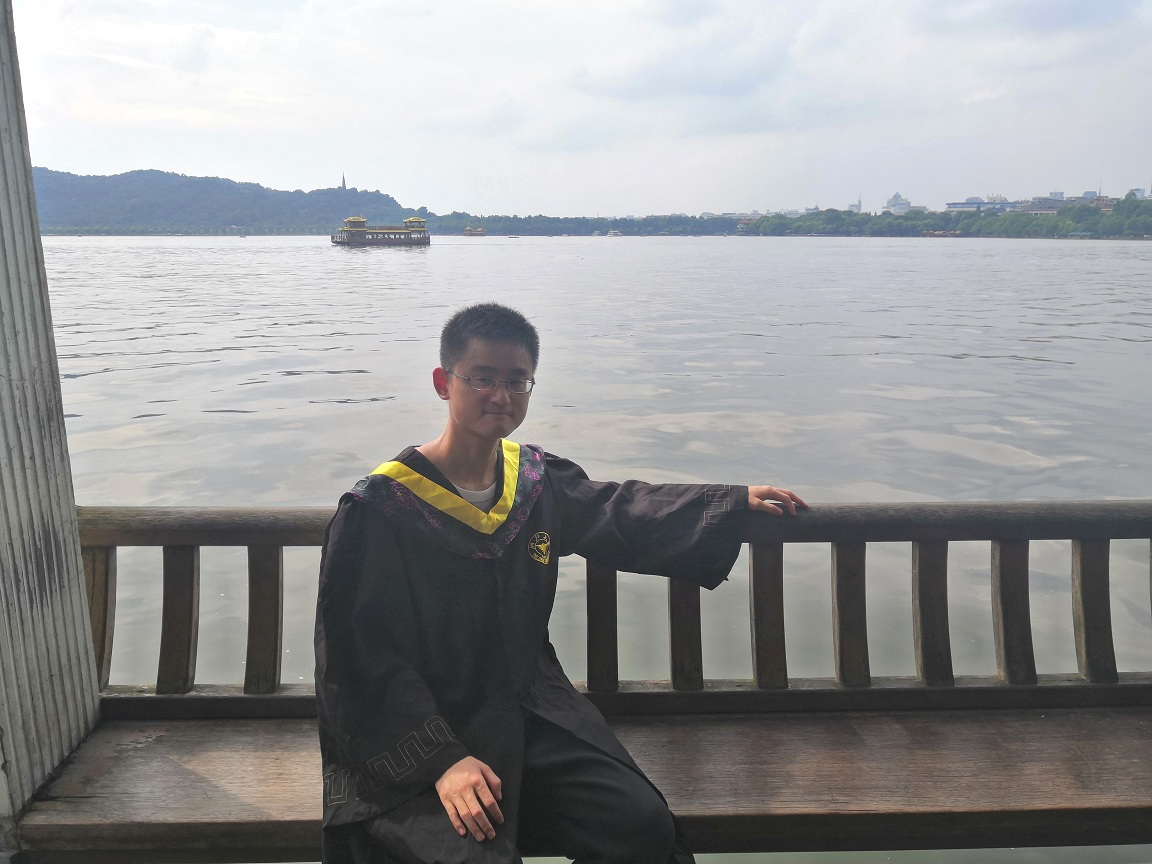
\includegraphics[width=7.5cm]{about2.jpg}
\end{center}
\end{tcolorbox}
\end{center}
\newpage
\ \\
\thispagestyle{empty}
\pagecolor{Yellow}


\end{document}







































